\chapter{Architettura della gamificazione}
Abbiamo quindi visto come costruire un sistema gamificato, quali sono i suoi elementi e che risultati può produrre. Cerchiamo ora di riorganizzare tutto questo in uno schema disegnando in generale una possibile architettura per la gamificazione.\\
Gli elementi principali di un sistema gamificato sono: gli obbiettivi, gli elementi di gioco, il feedback e analisi dei dati.

\begin{figure}[h!]
  \centerline{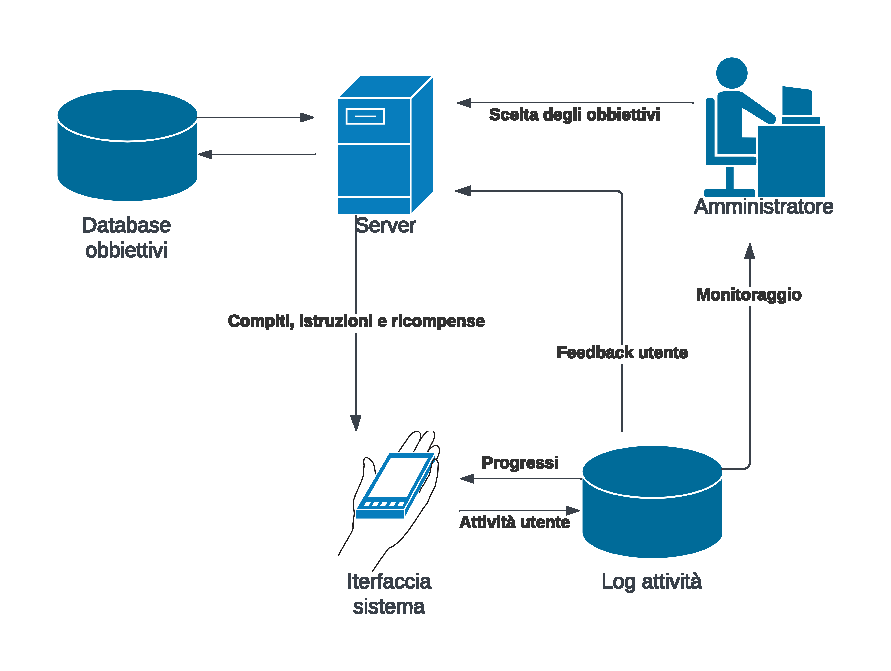
\includegraphics[angle=0]{figures/architettura.pdf}}
  \caption{Diagramma dell'architettura}
\end{figure}

L'architettura si promette di gestire un tipo di gamification che beneficia un'azienda (distinzione chiarita nella sezione 2.1 i tipi di gamification).
L'architettura ideata prevede l'utilizzo di un server che comunica un database contenente una lista di obbiettivi memorizzati tramite una mappa che denota una successione di step intermedi da raggiungere prima di considerare l'obbiettivo finale completato. Ad esempio un'azienda per aumentare le proprie vendite deve vendere più prodotti e quindi ne deve avere maggiore disponibilità, quindi deve anche aumentare la propria produzione. Una volta aumentata la produzione o vende di più ai propri clienti o trova più clienti ai quali vendere.\\
Questo server oltre a gestire la priorità dei compiti da raggiungere riceve dal log delle attività il feedback dell'utente e tramite quello assegna le ricompense che possono essere sotto forma di punti o badge nel caso si sia raggiungiuto un obbiettivo importante. \\
Per quanto riguarda la parte di front end il sistema prevede una distizione di due utenti. Un utente "amministratore" che beneficia dei risultati della gamification e l'utente "lavoratore", alle dipendenza o servizio dell'utente amministratore.

\section{Analisi dei requisiti}

Requisiti funzionali:
\begin{itemize}

  \item Il sistema deve permettere all'utente amministratore di creare gruppi di utenti in modo da dividerli in base al loro compito nell'organizzazione che si sta gamificando.

  \item Il sistema deve fornire all'utente amministratore interfaccia dove è possibile assegnare obbiettivi a singoli utenti o oppure un obbiettivo condiviso ad un gruppo di utenti.

  \item Il sistema deve permettere all'utente amministratore di visualizzare le attività dei vari utenti lavoratori.

  \item Il sistema deve fornire all'utente lavoratore un'iterfaccia dove visualizzare e segnare i propri progressi.

  \item Il sistema deve prevedere un sistema di ricompense dove è possibile spendere i punti che si sono accumulati.
\end{itemize}

Requisiti non funzionali:
\begin{itemize}

  \item Il sistema deve permettere all'utente amministratore disegnare mappe topologiche degli obbiettivi.

  \item Il sistema deve assegnare ad ogni azione degli utenti una ricompensa adatta.

  \item il sistema deve notificare l'utente amministratore quando gli utenti raggiungono un'obbiettivo oppure quando compiono azioni che tipicamente significano un allontanamento da esso.

  \item l'interfaccia dell'utente lavoratore deve fornire un report al server di tutte le operazioni degli utenti.
\end{itemize}

\begin{figure}[h!]
  \centerline{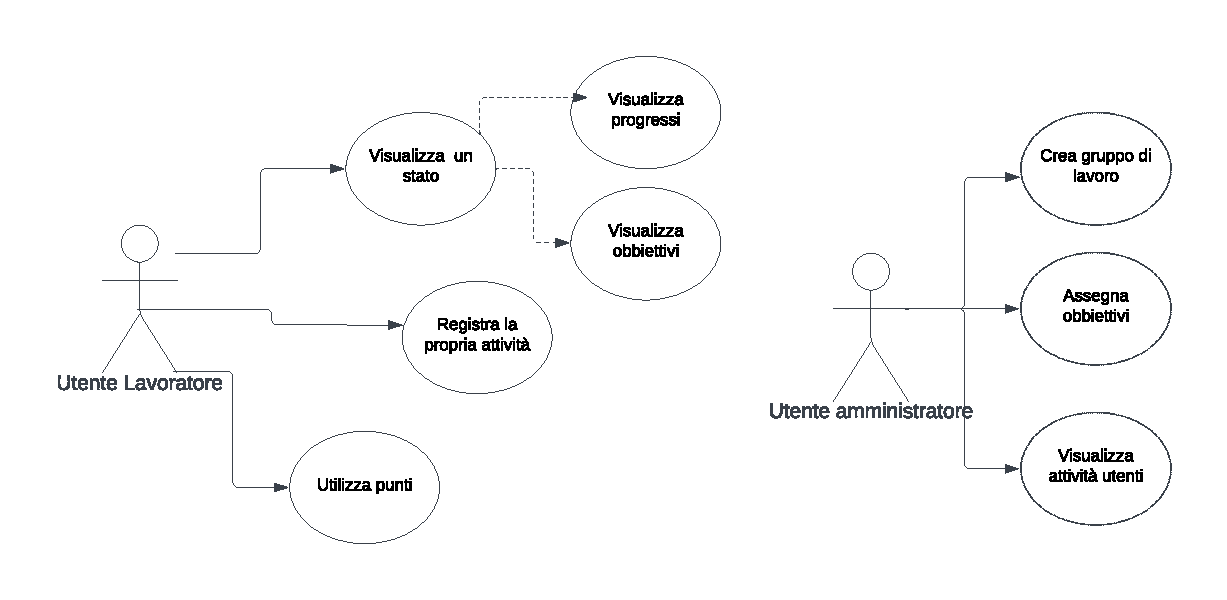
\includegraphics[angle=0]{figures/utenti.pdf}}
  \caption{Diagramma Use case}
\end{figure}

\section{Miglioramenti possibili}

È possibile introdurre dei miglioramenti alla architettura proposta implementando al suo interno tecnologie emergenti come quella dell'intelligenza artificiale.\\
Una possibile miglioria è quella di assistere l'utente amministratore nella creazione della mappa topologica. Si potrebbero salvare in un database tutte le mappe topologiche create da tutti gli utenti che hanno utilizzato il sistema e tramite machine learning proporre ad un utente che sta per creare una nuova mappa topologica una esempio che esso può modificare e aggiustare secondo i propri bisogni.\\
Un'altra possibile miglioria potrebbe essere quella di far gestire il sistema di ricompense all'intelligenza artificiale e regolarle in modo che motivino al meglio l'utente lavoratore per fargli raggiungere l'obbiettivo velocemente.\\
Un'ulteriore miglioria potrebbe essere quella di introdurre un'intelligenza artificiale che guidi l'utente amministratore alla creazione di un piano di gamificazione del proprio sistema in base alle esigenze del caso singolo.
